\documentclass[aps,reprint,amsmath,amssymb,showpacs,showkeys]{revtex4-1}% APS journal style
\usepackage{graphicx}% Include figure files
\usepackage{dcolumn}% Align table columns on decimal point
\usepackage{bm}% bold math
\usepackage{hyperref}% add hypertext capabilities
\usepackage{natbib}  % Package for Bibtex
%\usepackage{amsmath}  % Package for typesetting formulae
%\usepackage{amssymb}  % Package for some math symbols and fonts
\usepackage[justification=justified]{caption}
%\usepackage[caption=false]{subfig}
\usepackage{subcaption} % subfigure
\usepackage{amsopn}
\usepackage{float}
\usepackage{tikz}
\usetikzlibrary{shapes.geometric, arrows}
\tikzstyle{sqr2} = [rectangle, minimum width=3.5cm, minimum height=0.9cm, text centered, draw=black, fill=yellow!30]

\usepackage{ulem} % \sout function

\newcommand{\bt}[1]{\ensuremath{\mathbf{#1}}}  % bold math
%\newcommand{\bm}[1]{\mbox{\boldmath $#1$}}
\newcommand{\cb}{ \color{blue}}
\newcommand{\cred}{\color{red}}

\begin{document}
\graphicspath{{figures/}}	

% Define author, title, and date
\title[Stepping-stone sampling algorithm for evidence computation]{The stepping-stone sampling algorithm for calculating the evidence of gravitational wave models}

\author{Patricio Maturana Russel$^{1}$, Renate Meyer$^1$, John Veitch$^2$ and Nelson Christensen$^3$}
\affiliation{$^1$ Department of
  Statistics, University of Auckland, Auckland 1142, New Zealand \\
$^2$ Physics and Astronomy, University of Glasgow, United Kingdom\\
$^3$ ARTEMIS, Laboratoire de la C\^{o}te d'Azur, Nice, France}


\begin{abstract}
Bayesian statistical inference has become increasingly important for the analysis of observations from the Advanced LIGO and Advanced Virgo gravitational-wave detectors. To this end, iterative simulation techniques, in particular nested sampling and parallel tempering, have been implemented in the software library LALInference to sample from the posterior distribution of waveform parameters of compact binary coalescence events. Nested sampling was  mainly developed to calculate the evidence of a model but can produce posterior samples as a by-product. Thermodynamic integration is employed to calculate the evidence using samples generated by parallel tempering but has been found to be computationally demanding. Here we propose the stepping-stone sampling algorithm, originally proposed by Xie et al.\ (2011) in phylogenetics  and a special case of path sampling, as an alternative to thermodynamic integration.  The stepping-stone sampling algorithm is also based on samples from the power posteriors of parallel tempering but has  superior performance as less temperature steps and thus computational resources are needed to achieve the same accuracy.  We demonstrate its performance and computational costs in comparison to thermodynamic integration and nested sampling in a simulation study and a case study of computing the marginal likelihood of a binary black hole
model applied to simulated LIGO data {\cb John: please correct, not sure which data and model you have been using}.  To deal with the inadequate methods currently employed to estimate the standard errors of evidence estimates based on power posterior techniques, we propose a novel block bootstrap  approach and show its potential in our simulation study and LIGO application.
\end{abstract}

\pacs{04.30.-w, 02.50.-r, 05.45.Tp, 97.60.Bw}
\pacs{04.30.-w, 02.50.-r, 05.45.Tp, 97.60.Bw}

\keywords{thermodynamic integration, stepping-stone sampling, nested sampling, model selection, gravitational waves}




\maketitle

\section{Introduction}


%(Advanced LIGO \cite{aLIGO:2015},

% Advanced Virgo \cite{aVirgo:2015},

%and KAGRA \cite{KAGRA:2013}) 

%Littenberg and Cornish \cite{littenberg:2010} ,

%Littenberg \textit{et al} \cite{littenberg:2013},


%Littenberg and Cornish bayesline \cite{bayesline:2014}

%bayeswave \cite{bayeswave:2014}

%LALInference paper\cite{veitch:2015}

%\cite{veitch:2010}

%Nested sampling\cite{skilling:2006}%

{\cb
general review of evidence estimates that are used in the gravitational wave  literature\bigskip

- \textit{Discuss: importance of ``z"  
- how the uncertainty is estimated in power posterior methods}}

%RJMCMC Green \cite{green:1995}

The paper is structured as follows: Section II \ldots.



\section{Computation of Marginal Likelihood}

The \textit{evidence} or \textit{marginal likelihood} of a model  $M$ is a multi-dimensional integral defined as
\begin{align}
\label{eq:z}
z = \int_{\Theta}L(\bm{X}|\bm{\theta},M)\pi(\bm{\theta}|M) \text{d} \bm{\theta},
\end{align}
where $\bm{\theta} \in \Theta$ denotes the parameter vector, $\bm{X}$ the dataset, $L(\bm{X}|\bm{\theta},M)$  the likelihood function, and $\pi(\bm{\theta}|M)$  the prior density, assumed to be proper, i.e.\ $ \int_{\Theta}\pi(\bm{\theta}|M) \text{d} \bm{\theta}=1$.

In general, this integral (\ref{eq:z}) has no analytical solution and must be estimated using numerical methods.  Importance sampling techniques, in particular the arithmetic mean (AM) and harmonic mean (HM) methods,  provide the simplest way of estimating it \citep{Newton:Raftery:1994}.
% being the most popular among them the arithmetic (AM) and harmonic \citep[HM;][]{Newton:Raftery:1994} means.  
Let $\bm{\theta}_i, i=1,\ldots,n$ be samples from the prior, the AM estimator is an average of corresponding $n$ likelihood values:
\begin{align}
\label{eq:AM}
\widehat{z}_{AM} = \frac{1}{n}\sum_{i=1}^n L(\bm{X}|\bm{\theta}_i,M).
\end{align}
In general, high-likelihood areas are very small and  constitute a small fraction of the prior.  Therefore, unless $n$ is very large, the sample will not adequately represent these areas and yield a poor estimate.  The HM estimator is  based on samples 
$\bm{\theta}_i, i=1,\ldots,n$
 drawn from the posterior:
\begin{align}
\label{eq:HM}
\widehat{z}_{HM} = \left( \frac{1}{n}\sum_{i=1}^n \frac{1}{ L(\bm{X}|\bm{\theta}_i,M)} \right)^{-1}
\end{align}
i.e.\ the inverse of an average of inverse likelihood values or {\it harmonic mean} of likelihood values.
% Like the AM, HM also suffers from unrepresentative problems.  Those regions of low-likelihood values are rarely visited by the Markov chains.  The drawbacks of the HM estimator have been extensively documented in the literature of which we highlight it potentially infinite variance, that it is  insensitive to changes of the prior distribution, a general overestimation of the evidende, poor accuracy, unstable behaviour, and failure in high dimensions \citep{Lartillot:Philippe:2006, Newton:Raftery:1994, Xie:Lewis:Fan:Kuo:Chen:2011}.  %To sum up, importance sampling methods are not recommended for marginal likelihood estimation.

Therefore, the AM and HM estimators are not recommended because they produce unreliable estimates of the evidence even though they are easily calculated.   In this context, more complex approaches have been proposed, such as power posterior methods \cite{Xie:Lewis:Fan:Kuo:Chen:2011, Lartillot:Philippe:2006, Friel:2008, Neal:2001}.  These methods rely on a set of transitional distributions which connect the prior and the posterior, reminiscent of simulated annealing.  The geometric path is the most popular scheme used to connect these distributions and defines the \textit{power posterior density} as
\begin{align}\label{eq:powerposterior}
p_{\beta}(\bm{\theta}|\bm{X}, M) = \frac{L(\bm{X}|\bm{\theta},M)^{\beta}\pi(\bm{\theta}|M)}{z_{\beta}},
\end{align}
for $0\leq\beta\leq 1$, the inverse temperature, where $z_{\beta}$ is the normalizing constant, which is defined as $\int_{\Theta} L(\bm{X}|\bm{\theta},M)^{\beta}\pi(\bm{\theta}|M) \text{d}\bm{\theta}$. Note that the power posterior density turns into the prior and posterior for $\beta = 0$ and $\beta = 1$, respectively.   

Methods  that make use of samples from the power posteriors are much more accurate than HM as has been widely documented \citep{Lartillot:Philippe:2006, Newton:Raftery:1994, Xie:Lewis:Fan:Kuo:Chen:2011}, particularly in high dimensional problems.  Among these methods, thermodynamic integration (TI) \citep{Lartillot:Philippe:2006} is popular method to estimate the  evidence  of gravitational wave (GW) models, showing in general good performance.  Another method, widely applied in other fields such as phylogenetics is stepping-stone sampling (SS) algorithm \citep{Xie:Lewis:Fan:Kuo:Chen:2011}.  As this method
can provide many advantages over the TI estimate, it is important to explore the performance of  the SS estimator  for GW models as  to the best of our knowledge,  the  SS algorithm has not been used for evidence calculation in this context.

One of the drawbacks of power posterior methods is the significant computational cost required to produce a single evidence estimate as 
multiple Markov chains have to be run, one for each temperature.  Fortunately, since the usual practice to carry out parameter inference on GW models is parallel tempering, the samples at different temperatures are available and can be recycled in order to use these methods.  This is what software packages such as LALInference \citep{Veitch:2015} do in order to estimate the evidence.

However, as has been noticed in \cite{Veitch:2015}, TI might require a larger number of temperatures than the one needed for parameter estimation in order to achieve accurate estimates.  Note that the samples of chains  at  temperatures $T>1$ ($\beta<1$) are only used to aid the mixing of  the chain at $T=\beta=1$ whose stationary distribution is the posterior, and  are therefore discarded from the inference process.  In this context, SS algorithm seems very promising since  it requires fewer temperature steps than TI to provide accurate evidence estimates
as we will show in section \ref{sec:simulation}.     

Another method to estimate the evidence,  not based on power posteriors, is nested sampling (NS) \citep{Skilling:2006}.  This Bayesian algorithm has been successfully applied in diverse fields, such as astronomy \citep{Brewer:Donovan:2015} {\cb John: please add references}, cosmology \citep{Feroz:2009},  engineering \citep{Henderson:2017} and phylogenetics \citep{Maturana:2017b, Maturana:2018}. To estimate the evidence of GW models, NS has been implemented in the software package LALInference \citep{Veitch:2015}.  The method has the unique property of yielding an estimation of the uncertainty associated to the evidence estimate in a single run (subject to the independence of the samples), unlike power posterior methods. {\cb But this only holds for independent samples, not when running MCMC to sample from the
restricted prior as is done in practice}.

Alternatively, instead of estimating the evidence for each model being tested, a trans-dimensional Reversible Jump Markov chain Monte Carlo (RJMCMC) method can be used in order to explore the joint space of all models.  Then the probability for each model can be calculated simply by calculating the relative frequency of visits to each model by the Markov chain.  However, this exploration depends on tuning parameters which can be difficult to specify, leading to poor mixing of the Markov chain and subsequently to large statistical errors associated with the evidence estimates \citep{Cornish:2014}.

%{\cb I am not sure whether we need to include RJMCMC}.

Below we describe TI, SS and NS in more detail before comparing their performance in sections \ref{sec:simulation} and \ref{sec:LIGO}.




\subsection{Thermodynamic Integration}
Thermodynamic integration  or the more general path sampling \citep{Gelman:1998} make use of an auxiliary variable $\beta$, $0\leq \beta \leq 1$, to
define transitional distributions, namely the power posterior distributions defined in (\ref{eq:powerposterior}) in the case of TI, that provide a path from the prior ($\beta=0$) to the posterior distribution ($\beta=1$). By explicitly denoting the evidence $z_\beta$ as a function of $\beta$ by
\[z(\bm{X}|\beta)=\int_{\Theta} L(\bm{X}|\bm{\theta},M)^{\beta}\pi(\bm{\theta}|M) \text{d}\bm{\theta},\]
the log marginal likelihood has the representation as the integral over the 1-dimensional parameter $\beta$ of half the mean deviance where the expectation is taken with respect to the power posterior:
\begin{equation}\label{eq:TI}
\log(z)=\log\left( \frac{z(\bm{X}|\beta=1)}{z(\bm{X}|\beta=0)}\right)=\int_0^1 E_{\beta} \left[ \log(p(\bm{X}|\bm{\theta},M)\right]\text{d}\beta.
\end{equation}
Representation (\ref{eq:TI}) follows by integration from
\begin{align*}
&\frac{\partial}{\partial\beta} \log(z(\bm{X}|\beta)) = \frac{1}{z(\bm{X}|\beta)} \frac{\partial}{\partial\beta} z(\bm{X}|\beta)\\
&= \frac{1}{z(\bm{X}|\beta)} \frac{\partial}{\partial\beta}\int_{\Theta} L(\bm{X}|\bm{\theta},M)^{\beta}\pi(\bm{\theta}|M) \text{d}\bm{\theta}\\
&=  \frac{1}{z(\bm{X}|\beta)} \int_{\Theta}  L(\bm{X}|\bm{\theta},M)^{\beta}\log(L(\bm{X}|\bm{\theta},M)) \pi(\bm{\theta}|M) \text{d}\bm{\theta}\\
&=  \int_{\Theta}   \frac{L(\bm{X}|\bm{\theta},M)^{\beta}\pi(\bm{\theta}|M)}{z_{\beta}} \log(L(\bm{X}|\bm{\theta},M))\text{d}\bm{\theta}\\
&= E_{\beta} \left[ \log(L(\bm{X}|\bm{\theta},M)\right].
\end{align*}
The samples from the parallel tempered chains for different values of $\beta$ provide samples from the power posteriors and the
expectation $E_{\beta}\left[ \log(L(\bm{X}|\bm{\theta},M)\right]$ is then estimated by the sample average. The integral
in equation (\ref{eq:TI}) is then approximated by numerical integration, e.g. using the trapezoidal or Simpson's rule.


\subsection{Stepping-stone Sampling Algorithm}
Stepping-stone sampling is another method to estimate the marginal likelihood.  It has been widely used by the phylogenetic community where it was proposed by \cite{Xie:Lewis:Fan:Kuo:Chen:2011}.  SS works basically by mixing elements from importance sampling and simulated annealing methods.  This method relies on the same sampling scheme required by TI.  Therefore, its implementation in any software package where TI or parallel tempering has already been implemented should be straightforward.  SS has the advantage of requiring fewer path steps than TI to accurately estimate  the marginal likelihood and yielding a less-biased estimator as demonstrated in section \ref{sec:simulation}.

The marginal likelihood can be seen as the ratio $z = z_1/z_0$, where $z_0 = 1$ since the prior is assumed to be proper.  The direct calculation of this ratio via importance sampling is not reliable because the distributions involved in the numerator and denominator (posterior and prior, respectively) are, in general, quite different.  To solve this problem, SS expands this ratio in a telescope product of $K$ ratios of normalizing constants of the transitional distributions \cite{Neal:1993}, that~is
\begin{align*}
\label{eq:SS_ratios}
z = \frac{z_{1}}{z_{0}} = \frac{z_{\beta_{1}}}{z_{\beta_{0}}}\frac{z_{\beta_{2}}}{z_{\beta_{1}}} \dots
\frac{z_{\beta_{K-2}}}{z_{\beta_{K-3}}} \frac{z_{\beta_{K-1}}}{z_{\beta_{K-2}}} = \prod_{k=1}^{K-1} \frac{z_{\beta_{k}}}{z_{\beta_{k-1}}} = \prod_{k=1}^{K-1} r_k,
\end{align*}
for $\beta_0 = 0 < \beta_1 < \dots < \beta_{K-2}<\beta_{K-1} =~1$, being the sequence of inverse temperatures, where $r_k=z_{\beta_k}/z_{\beta_{k-1}}$.  These individual intermittent ratios can be estimated  with higher accuracy than
$\frac{z_1}{z_0}$ because the  distributions in the
numerator and denominator are generally quite similar when using a reasonable number of temperatures $K$.  In this situation the importance sampling method works well. 

SS estimates each ratio $r_k$ by importance sampling using $p_{\beta_{k-1}}$ as importance sampling distribution.  This is a suitable distribution because it has heavier tails than $p_{\beta_{k}}$ which leads to an efficient estimate of $r_k$.  In this manner, it avoids estimating from the posterior distribution, making it slightly less expensive computationally than TI for the same number of path steps.  The estimation of each ratio is based on the identity
\begin{align*}
r_k = \frac{z_{\beta_{k}}}{z_{\beta_{k-1}}} &= \int_{\Theta}\frac{L(\bm{X}|\bm{\theta},M)^{\beta_{k \quad}}}{L(\bm{X}|\bm{\theta},M)^{\beta_{k-1}}} \: p_{\beta_{k-1}}(\bm{\theta}|\bm{X},M) \text{d}\bm{\theta}, 
%&=\mathds{E}_{p_{\beta_{k-1}}}\bigg[ \frac{q_{\beta_{k}}(\bm{\theta})}{q_{\beta_{k-1}}(\bm{\theta})} \bigg].
\end{align*}
which is estimated by its unbiased MC estimator
\begin{align*}
\widehat{r}_k = \frac{1}{n} \sum_{i = 1}^{n}  L( \bm X | \bm{\theta}_{\!\beta_{k-1}}^{i}, M)^{\beta_{k}-\beta_{k-1}},
\end{align*}
where $\bm{\theta}_{\!\beta_{k-1}}^{1}, \dots, \bm{\theta}_{\!\beta_{k-1}}^{n}$ are drawn from $p_{\beta_{k-1}}$ with $k = 1, \dots, K-1$. 

Therefore,  the SS estimate of the marginal likelihood is defined as 
\begin{align*}
\widehat{z} &= \prod_{k=1}^{K-1}\frac{1}{n} \sum_{i = 1}^{n}  L( \bm X | \bm{\theta}_{\!\beta_{k-1}}^{i}, M)^{\beta_{k}-\beta_{k-1}},
\end{align*}
with log-version
\begin{align*}
\log\widehat{z} &= \sum_{k=1}^{K-1} \log \sum_{i = 1}^{n}  L( \bm X | \bm{\theta}_{\!\beta_{k-1}}^{i}, M)^{\beta_{k}-\beta_{k-1}} - (K-1) \log n.
\end{align*}
Although $\widehat{z}$ is an unbiased, the log transformation introduces a bias which can be alleviated by increasing $K$ \citep{Xie:Lewis:Fan:Kuo:Chen:2011}.

The performance of this method depends naturally on its specifications such as the number of transitional distributions and number of samples from each of them ($K$ and $n$, respectively).  The dispersal of the $\beta$ values has also a strong influence, even more so in TI (see \cite{Xie:Lewis:Fan:Kuo:Chen:2011} and our simulation study below).  Along these lines, \cite{Xie:Lewis:Fan:Kuo:Chen:2011} proposed to spread the $\beta$ values according to the evenly spaced quantiles of a Beta(0.3, 1) distribution.  This distribution is right skewed, thereby putting half of the $\beta$ values below 0.1 where most of the variability  is found.    

SS is closely related to annealed importance sampling \citep[][]{Neal:2001}.  The latter utilizes the same product of ratios, but instead of estimating each ratio separately, it estimates the entire product via importance sampling, that is the whole telescope product is evaluated multiple times and then the these values are averaged \citep{Maturana:2017}.  For the particular case of $K = 2$, that is considering only the prior, both methods reduce to the arithmetic mean, and for $n =1$, they are equivalent.   


\subsection{Nested Sampling}

NS transforms the multidimensional integral defined in~\eqref{eq:z}, by making use of a property of positive random variables (see~\cite{Maturana:2017b} for more details), into a one-dimensional one that utilizes a function that relates the prior with the likelihood as 
\begin{align*}
z = \int_{0}^{1} L(\xi)\text{d}\xi, 
\end{align*}
where $L$ is the likelihood as a function of the prior volume~$\xi$.  This function can be read as the proportion of prior volume $\xi$ with likelihood values greater than $L(\xi)$. 

This likelihood is a non-increasing function over the unit range.  For a given decreasing sequence of $\xi$-values and an increasing sequence of $L$-values, the marginal likelihood can be estimated using, for instance, the trapezium rule
\begin{align*}
\widehat{z}_{NS} = \sum_{i=1}^{K} \dfrac{1}{2}(\xi_{i-1} - \xi_{i+1})L_i,
\end{align*}
where $0 < \xi_{K+1} < \xi_{K} < \cdots < \xi_1<\xi_0 = 1$.

NS explores the parameter space from the prior toward those areas of high likelihood values over time.  For this, a set of $N$ points, called \textit{live} points, are drawn independently from the prior.  The point $\bm{\theta}_1$ with the lowest likelihood associated to these points is detected and the latter is registered as $L_1$.  Then, this point $\bm{\theta}_1$ is replaced by a new one $\bm{\theta}^*$ drawn from the prior but restricted to have a greater likelihood, that is $L(\bm{\theta}^*) > L(\bm{\theta}_1)$.  This procedure is repeated until a given stopping criterion is satisfied.  Thus, an increasing sequence of likelihood values $L_1, \dots, L_K$ is generated.

Even though the $\xi$-values cannot be measured precisely, the nature of this algorithm allows to estimate them.  The $\xi$-sequence can be defined as 
\begin{align*}
\xi_1 = u_1,\: \xi_2 = u_2 \xi_1, \dots,\: \xi_K = u_K \xi_{K-1},
\end{align*}
where $u_i\sim\text{Beta}(N,1)$.  The geometric mean is the most common method to estimate the $u$-values, which yields
\begin{align*}
\xi_i = e^{-i/N}.
\end{align*}

The nature of NS algorithm also allows to estimate the uncertainty in a single run as 
\begin{equation}\label{eq:SDNS}
\text{SD}(\log z) = \sqrt{\dfrac{H}{N}},
\end{equation}
where $H$ is the negative entropy.  Alternatively, for a fixed sequence of likelihood values and multiple sequence of $\xi$-values, generated from different  $u\!\sim\!\text{Beta}(N,1)$ values, a distribution of marginal likelihood estimates can be generated and subsequently the uncertainty can be estimated.  NS results are valid if and only if the samples drawn at each iteration are independent.

\bigskip


\section{Estimation of the MC Standard Error of the Evidence}
The point estimate of the evidence  is not sufficient if we want to compare the  performance of different types of evidence estimates.   We
need  to have a measure of the Monte Carlo standard error of the evidence estimates.  In the NS case, the algorithm provides direct ways of calculating its standard error from  a single run as given in (\ref{eq:SDNS}).  However, power posterior methods lack a reliable direct way of calculating the standard error of the evidence.  In \cite{Lartillot:Philippe:2006} and \cite{Xie:Lewis:Fan:Kuo:Chen:2011}, the authors proposed estimates which rely on the  independence of the samples in the Markov chains at different temperatures, an assumption that is not met  in general.  Practitioners opt for the standard procedure of repeating the analysis multiple times and then calculating the standard error.  This brute force technique can be very costly and is in some cases computationally not viable.  Alternatively, some estimate the error internally in a single run, that is by re-sampling independently the Markov chains in order to generate multiple evidence estimates.  However, this approach does not consider the potential autocorrelation in the samples, leading to wrong estimates.  Here, we propose the use of a block bootstrap method for multivariate time series, which accounts for  the autocorrelation between the samples within a Markov chain at a fixed
temperature and the cross-correlation between parallel chains at different temperatures.
	
{\cb Cornish and Littenberg (2015) \citep{Cornish:2014} estimate TI error based on RJMCMC results. Maybe we should mention it.}
	

%\subsection{Block bootstrap method}	
Bootstrap is a resampling procedure proposed by \cite{Efron:1979}, initially for independent variables and later generalized by several authors.  \cite{Kunsch:1989} proposed an extension for the case of time series, which differs from the original algorithm by allowing the sampling in blocks.  The method is known as \textit{moving block bootstrap}, in short MBB.  This allows to take into account the presence of dependence in the data.

Let $X_1, \dots, X_n$ be the observed values from a sequence of stationary random variables, in our case, a Markov chain.  Define the overlapping blocks  $B_i = (X_i, ,\dots,X_{i+\ell-1})$ of length $\ell$, for $1\leq i \leq n-\ell + 1$ and $1 \leq \ell \leq n$, that is
\begin{align*}
B_1 &= (X_1, X_2, X_3, \dots, X_{\ell}) \\
B_2 &= (X_2, X_3, X_4, \dots, X_{\ell + 1}) \\
&\:\:\vdots\\
B_m &= (X_{n-\ell +1}, \dots, X_{n}), 
\end{align*} 
where $m = n - \ell +1$.  MBB works by resampling randomly $b$ blocks (for didactic reasons, suppose that $b = n/\ell$) and concatenating them in order to form a set of bootstrap observations $X^*_1,\dots,X^*_n$.  For $\ell = 1$, the original bootstrap method for i.i.d. data is recovered.  This procedure is repeated as usual, generating the distribution of the statistic of interest, in our case the marginal likelihood.  In the general case that $n$ is not a multiple of $\ell$, we can concatenate the random sample of $b$ block bootstraps, where $b$ is $n/\ell$ rounded up, and discard the leftover points $X^*_{n+1}, \dots, X^*_{b\ell}$, such that the bootstrap observation set has length $n$, as the original dataset.

Variants of this method can be found in \cite{Lahiri:2003}, such as \textit{stationary bootstrap}, where the block length follows a geometric distribution;  \textit{nonoverlapping block bootstrap}, which as its name say, considers nonoverlapping blocks; and \textit{circular block bootstrap}, which increases the original dataset with the first $\ell - 1$ observations in order to give equal weights to all of them. 

In the context of parallel tempering, in which case there are multiple Markov chains, we can generate the bootstrap observations using the same scheme for all the chains.  For instance, assuming equal chain lengths, a bootstrap observation set for a Markov chain consisting in $(B_6,B_4,B_2)$, can be replicated across the other chains.  This procedure takes into account the potential autocorrelation within the chains and the cross-correlation between the chains due to the swaps in parallel tempering sampling.  This is the approach applied in our examples.

\section{Simulation Study} \label{sec:simulation}
We consider a simple Gaussian model used by \cite{Lartillot:Philippe:2006} to test TI and compare it to the harmonic mean method.  Here, it is used to compare SS to TI.  In  addition, we assess the error estimate via the moving block bootstrap method and compare it to the empirical calculation of the error.  

The model is parametrized by a vector $\bm{x} = (x_1,x_2, \dots, x_d)$ of dimension $d$. The prior on $\bm x$ is a product of independent standard normal distributions on each $x_i$, for $i = 1, \dots,d$.  The likelihood is 
\begin{align*}
L(\bm{x}) = \prod_{i=1}^{d} e^{- \frac{x_i^2}{2v}},
\end{align*}
where $v$ is a parameter.  Doing some calculations, it is easy to see that the posterior distribution is given by a product of independent $\text{N}(0, v/(1+v))$ distributions, and therefore, its marginal likelihood has an analytical solution, which is $z = (v/(1+v))^{d/2}$.  The power posterior or transitional distributions are given by a product of independent  $\text{N}(0,v/(v+\beta))$ distributions.  All the involved distributions are Gaussians, so the sampling required to calculate TI and SS is straightforward.  However, we use the Metropolis algorithm to sample these densities and thus allow a certain degree of autocorrelation in the samples, making the analysis more realistic in an evidence estimation context.  The Markov chains have a lag of around 18 on average.  In addition, we consider independent samples to asses mbb performance in the context of error estimation.  

\begin{figure}[]
	\begin{subfigure}{0.50\textwidth}
		\centering 
		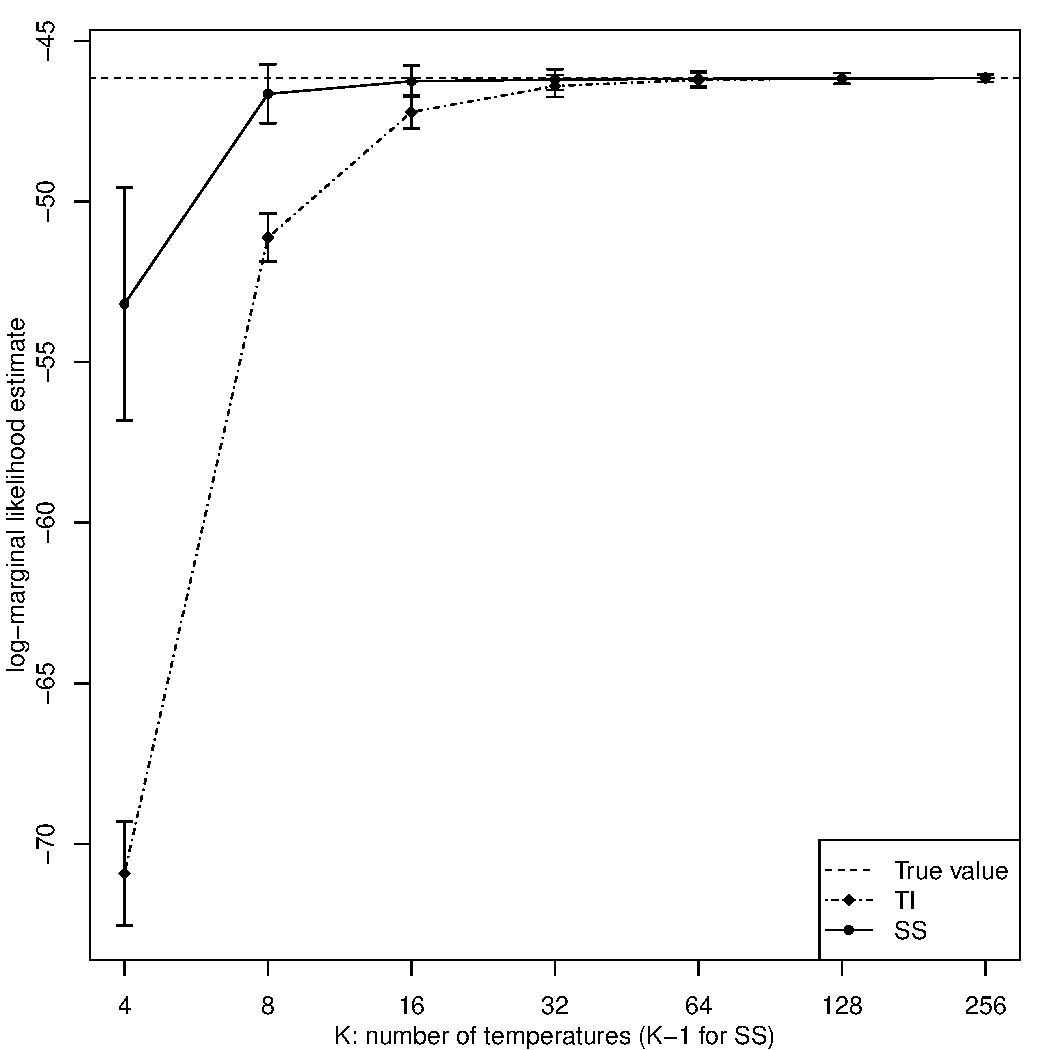
\includegraphics[scale=0.45,clip=true,angle=0]{toyExBetaTemp.pdf}
		\caption{$\beta$ values spread according to evenly spaced quantiles of a Beta(0.3, 1) distribution.}
		\label{fig1a}
	\end{subfigure}
	\begin{subfigure}{0.50\textwidth}
		\centering 
		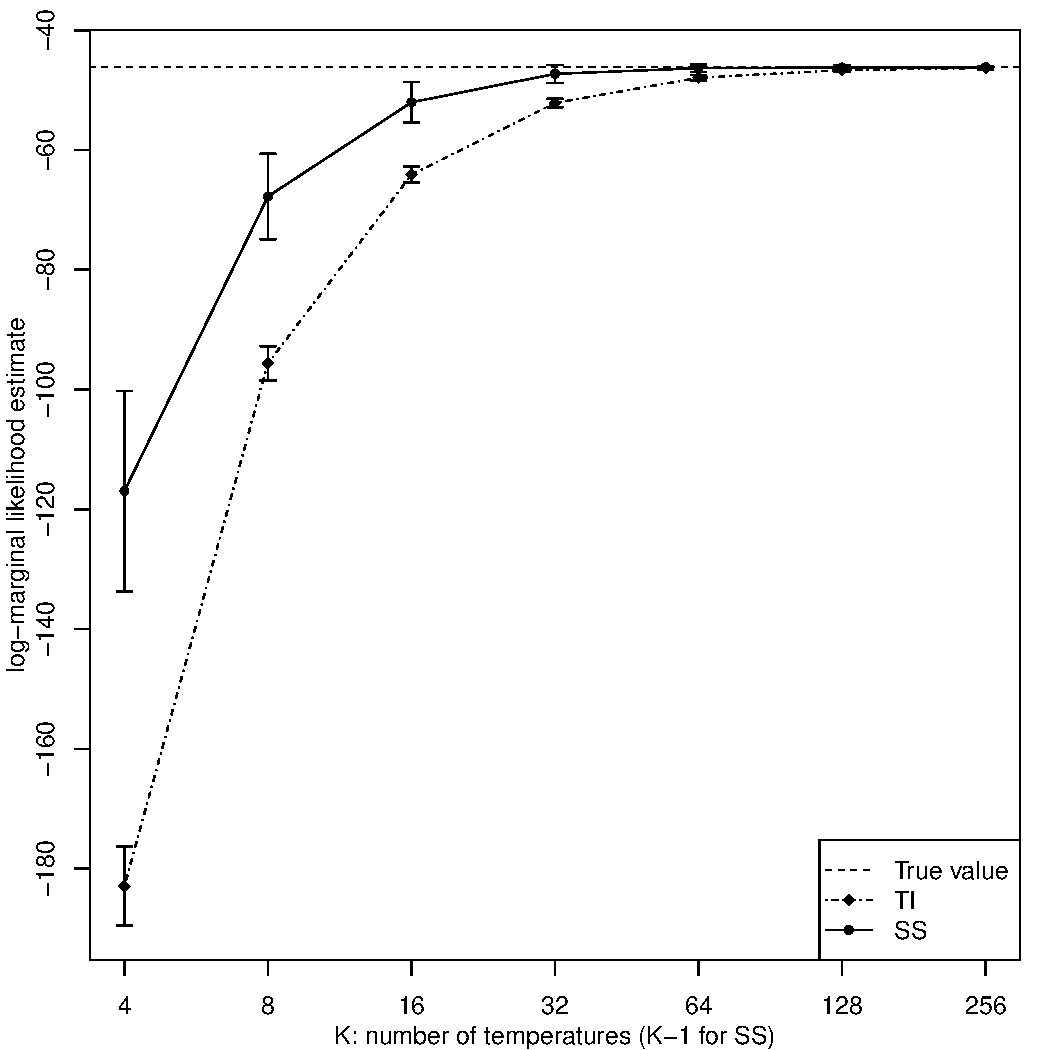
\includegraphics[scale=0.45,clip=true,angle=0]{toyExUnifTemp.pdf}
		\caption{$\beta$ values equally spaced between 0 and 1.} %\vspace{1.25em} }
		\label{fig1b}
	\end{subfigure}	
	\caption{Log-marginal likelihood estimates as a function of the number of temperatures $K$ for the Gaussian model.  Error bars depict $\pm1$ standard error based on 1000 independent MCMC analyses.}		
	\label{fig1}
\end{figure}

\subsection{Evidence estimate}

We consider the following model specifications: $v = 0.01$ and $d = 20$.  This yields a log-marginal likelihood value $-46.15$.  The analysis is performed for $n = 1000$ and $K = 4, 8, 16, 32, 64, 128, 256$.  Strictly speaking, SS uses $K-1$ temperatures, since does not require samples from the posterior.  For the arrangement of the $\beta$ values, we test two approaches: evenly spaced values from 0 to 1, and values spread according to evenly spaced quantiles of a $\text{Beta}(0.3, 1)$ distribution.  The MCMC analysis is replicated 1000 times (with different random seeds) in order to calculate the error associated with the estimates.  The same power posterior samples are used to estimate SS and TI. %{\cb more explicit: run the MCMC 1000 times with different starting values or random seeds??}

Figures~\ref{fig1a} and \ref{fig1b} display the results. It can be clearly noticed in both cases that SS requires less temperatures than TI to produce estimates around the true value.  For the case the $\beta$ values are calculated according to a Uniform(0,1), Figure~\ref{fig1b}, TI fails dramatically for low number of temperatures, whereas SS, even though it fails too, its estimates are closer to the true value.  For $K=4$, TI is more than 130 units away from the true value.  This shows that TI is more sensitive to the distribution of the temperatures as was similarly shown by \cite{Xie:Lewis:Fan:Kuo:Chen:2011}.

Both methods improve their performance when most of the computational effort is allocated in sampling in power posterior distributions near the prior, that is for hight temperatures.  This is the effect of the Beta(0.3, 1) distribution, which allows that half of the $\beta$ values are less than 0.1.  The results for this case are displayed in Figure~\ref{fig1a}.  Even though TI improves its performance considerably, it can not outperform SS, which still needs fewer step temperatures to produce estimates around the true value. 

\subsection{Standard error estimate}
\label{subsec:SDest}

Based in the case that the $\beta$ values follow a Beta(0.3, 1) distribution, we study the performance of the MBB method for estimating the evidence error.  For this, we calculate the standard error from the 1000 independent evidence estimates used in the previous analysis and compare it to the values calculated via MBB for different block lengths, $\ell = 1, 10, 30, 50, 100, 200, 300$.  

\begin{figure}[]
	\begin{subfigure}{0.50\textwidth}
	\centering 
	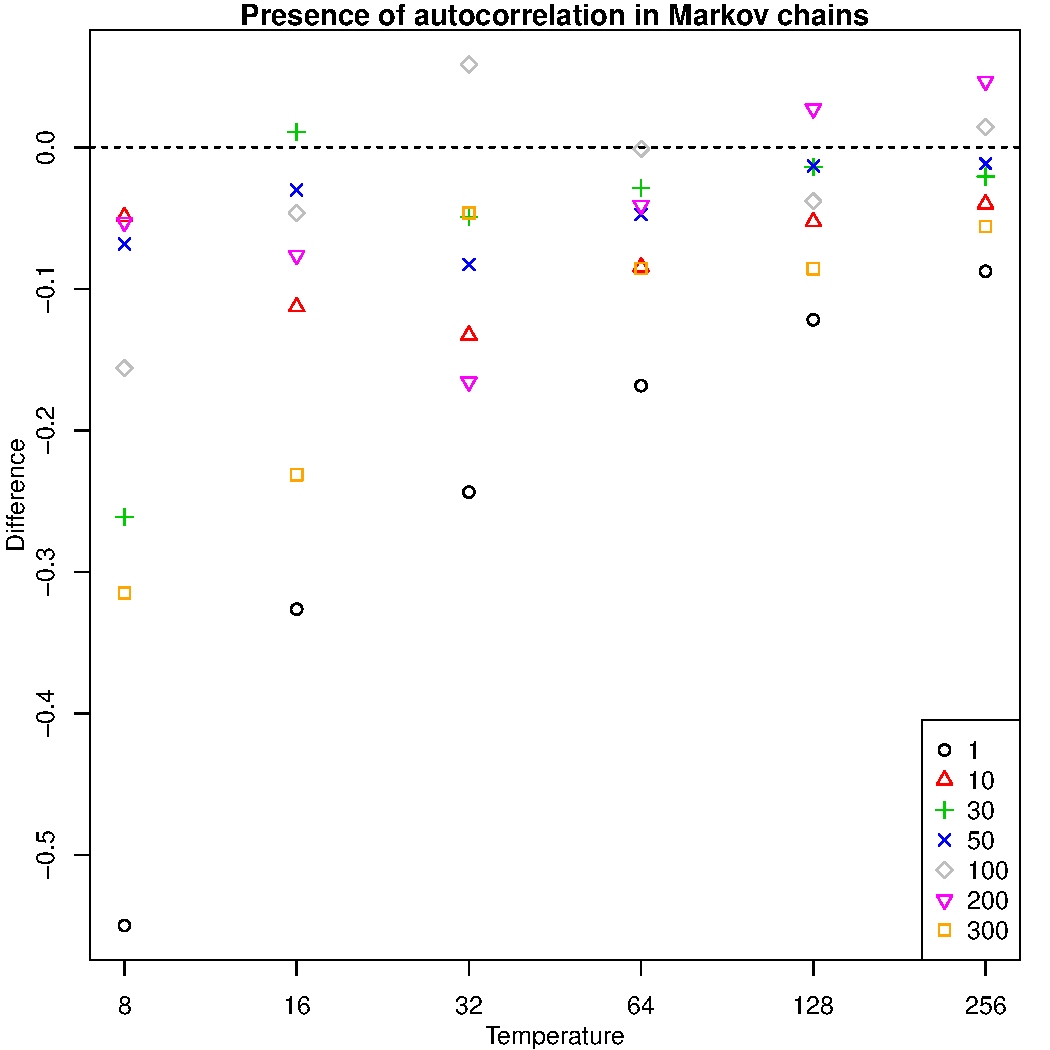
\includegraphics[scale=0.45,clip=true,angle=0]{ErrorEstimates_DepMC.pdf}
	\caption{The Markov chains contain a degree of autocorrelation.}
	\label{fig2a}
	\end{subfigure}
	\begin{subfigure}{0.50\textwidth}
	\centering 
	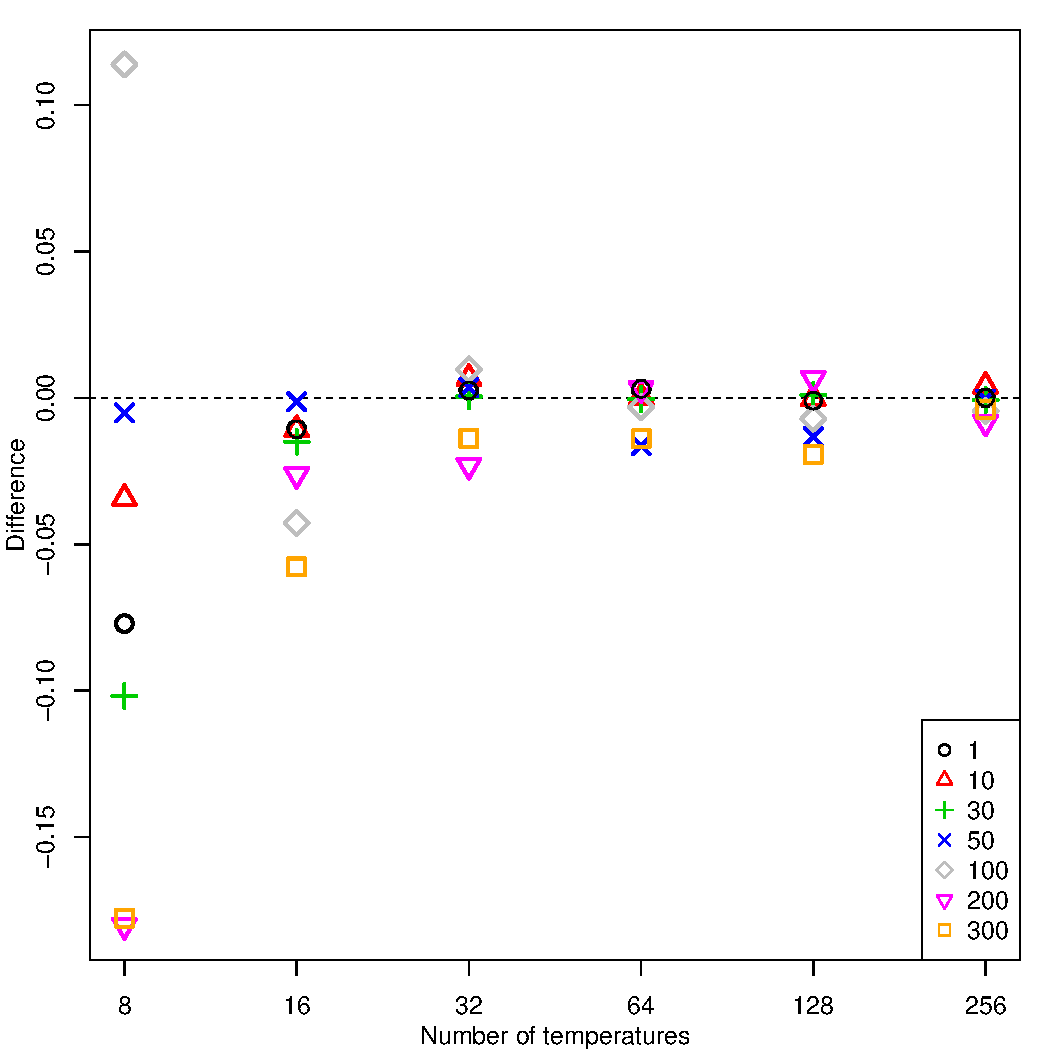
\includegraphics[scale=0.45,clip=true,angle=0]{ErrorEstimates_IndMC.pdf}
	\caption{The samples in the Markov chain are completely independent.}
	\label{fig2b}
	\end{subfigure}
	\caption{Standard error of independent evidence estimates versus the one calculated via MBB.  The numbers inside the plot stand for $K$, number of temperatures.  The legend describes the different block lengths used in MBB.}
	\label{fig2}
\end{figure}

The results are shown in Figure~\ref{fig2a}.  The case $\ell = 1$ is the original bootstrap method, which is used frequently for power posterior methods, but which ignores the dependence in the sampled values of the Markov chain.  It is obvious that in the simple bootstrap with block length $\ell=1$, the standard error is severely underestimated. On the other hand, the standard error estimates  improved significantly using 
the MBB with larger block lengths, but still some underestimate  the standard error.  However, this example is an extreme case of highly correlated Markov chains.  

We have also performed the analysis in the ideal case that the samples in the Markov chains are completely independent.  The result are displayed in Figure~\ref{fig2b}.  In this case, the standard bootstrap method, that is $\ell = 1$, is sufficient to estimate the standard error reasonable. Large block lengths cause, in general, a slight underestimation in the case of low temperature numbers, but as the number of temperatures increases, the estimates are located around the empirical error estimates and less dispersed.

%{\cb For independent samples, we have no autocorrelation, just cross-correlation between chains due to the swaps. I would guess that for that case, $\ell=1$ would work fine as long as we are resampling the same blocks in the parallel chains. I think we should explain that in the text in Section III as well.}


\section{Application to LIGO Data} \label{sec:LIGO}
{\cb John: Some description of the data etc

Could/should we also calculate the marginal likelihood here for the same data but for a model without signal present and calculate the BF and compare?

Include a comparison of TI and SS to the nested sampling estimate}

\section{Discussion}
SS is a method to estimate the marginal likelihood which has great popularity in phylogenetics where has shown to work well.  It requires slightly less computational cost than TI to yield a less biased estimator.  For our simple Gaussian model, we have shown that it is less sensitive to the disposal of the $\beta$ values and the number of power posterior distributions.  To the best of our knowledge, it has not been applied into gravitational wave models yet.  Its implementation in this context should be straightforward since its main complexity lies with sampling from the power posterior, like TI.  However, this can be done by using the parallel tempering method, which has been widely implemented in software packages in the gravitational wave context. 

The performance of SS depends on its specifications, such as $n$, $K$ and the distribution of the $\beta$ values.  In addition, it depends on how different the prior and the posterior are.  To avoid the dependence on the prior distribution, an extension of SS has been proposed, which is known as generalized steppingstone sampling \citep[GSS;][]{fan:2011}.  This method makes use of a reference distribution which aims to shorten the distance between the prior and the posterior.  Even though it requires posterior samples to construct the reference distribution, it is much more accurate than its simple version and requires less steps to yield the same accuracy.  This happens only if the reference distribution is a reasonable approximation of the posterior, otherwise it can dramatically fail \citep{Maturana:2017b}.  

One of the drawbacks of power posterior methods is the lack of a direct procedure to estimate the error associated to the evidence estimation.  In practice, the evidence is estimated multiple times in order to estimate empirically its standard error.  This procedure might be highly expensive.  Alternatively, some use the standard bootstrap method.
It is much cheaper than the first approach, but it does not have the power of taking into account any kind of dependency within and between the Markov chains.  We have proposed a moving block bootstrap method (MBB).  This approach has the power of taking into account potential autocorrelation within the chains and cross-correlation between chains.  We showed in Example~\ref{subsec:SDest} that standard bootstrap underestimates severally the empirical error in the presence of autocorrelation in the Markov chains.  On the other hand, the MBB method improves significantly the estimates.   

{\cb importance here demonstrated for compact binary inspirals but point out that algorithm is important as well for astrophysical and cosmological model selection}. 

\begin{acknowledgements}
  We thank Claudia Kirch for helpful discussions on the block-bootstrap for time series.  We also thank the New Zealand eScience Infrastructure (NeSI) for their high performance computing facilities, and the Centre for eResearch at the University of Auckland for their technical support. PM's and RM's work is supported by Grant 3714568 from the University of Auckland Faculty Research Development Fund and the DFG Grant KI 1443/3-1, and NC's work by NSF grants PHY-1204371 and PHY-1505373. This paper has been given LIGO Document Number xxxxx.  All analysis was conducted in \textsf{R}, an open-source statistical software available on \textsf{CRAN} (cran.r-project.org) and LALInference.
\end{acknowledgements}
\pagebreak

%%%%%%%%%%


\bibliographystyle{apsrev4-1}

\bibliography{PRDSS}

\end{document}

\begin{thebibliography}{10}



\bibitem{aLIGO:2015} The LIGO Scientific Collaboration, Advanced LIGO,
  \textit{Classical and Quantum Gravity}, \textbf{32}, 074001 (2015).

\bibitem{aVirgo:2015} F.~Acernese \textit{et al}, Advanced Virgo: a
  second-generation interferometric gravitational wave detector,
  \textit{Classical and Quantum Gravity}, \textbf{32}, 024001 (2015).

\bibitem{KAGRA:2013} Y.~Aso, Y.~Michimura, K.~Somiya, M.~Ando,
  O.~Miyakawa, T.~Sekiguchi, D.~Tatsumi, and H.~Yamamoto,
  Interferometer design of the KAGRA gravitational wave detector,
  \textit{Physical Review D}, \textbf{88}, 043007 (2013).

\bibitem{littenberg:2013} T.~B.~Littenberg, M.~Coughlin, B.~Farr, and
  W.~M.~Farr, Fortifying the characterization of binary mergers in
  LIGO data, \textit{Physical Review D}, \textbf{88}, 084044 (2013).

\bibitem{christensen:2010} N.~Christensen (for the LIGO Scientific
  Collaboration and the Virgo Collaboration), LIGO S6 detector
  characterization studies, \textit{Classical and Quantum Gravity},
  \textbf{27}, 194010 (2010).

\bibitem{lsc:2013} J.~Aasi \textit{et al}, Parameter estimation for
  compact binary coalescence signals with the first generation
  gravitational-wave detector network, \textit{Physical Review D},
  \textbf{88}, 062001 (2013).

\bibitem{bayesline:2014} T.~B.~Littenberg, and N.~J.~Cornish, Bayesian
  inference for spectral estimation of gravitational wave detector
  noise, \textit{Physical Review D}, \textbf{91}, 084034 (2015).

\bibitem{abadie:2012} The LIGO Scientific Collaboration and the Virgo
  Collaboration, Sensitivity achieved by the LIGO and Virgo
  gravitational wave detectors during LIGO's sixth and Virgo's second
  and third science runs, arXiv:1203.2674 [gr-qc] (2012).

\bibitem{sintes:1998} A.~M.~Sintes, and B.~F.~Schutz, Coherent line
  removal: Filtering out harmonic related line interference from
  experimental data, with application to gravitational wave detectors,
  \textit{Physical Review D}, \textbf{58}, 122003 (1998).

\bibitem{finn:2001} L.~S.~Finn, and S.~Mukherjee, Data conditioning
  for gravitational wave detectors: A Kalman filter for regressing
  suspension violin modes, \textit{Physical Review D}, \textbf{63},
  062004 (2001).

\bibitem{roever:2011a} C.~R\"{o}ver, R.~Meyer, and N.~Christensen,
  Modelling coloured residual noise in gravitational-wave signal
  processing, \textit{Classical and Quantum Gravity}, \textbf{28},
  015010 (2011).

\bibitem{whittle:1957} P.~Whittle, Curve and periodogram smoothing,
  \textit{Journal of the Royal Statistical Society: Series B
    (Methodological)}, \textbf{19}, 38--63 (1957).

\bibitem{roever:2011b} C.~R\"{o}ver, Student-$t$ based filter for
  robust signal detection, \textit{Physical Review D}, \textbf{84},
  122004 (2011).

\bibitem{littenberg:2010} T.~B.~Littenberg, and N.~J.~Cornish,
  Separating gravitational wave signals from instrument artifacts,
  \textit{Physical Review D}, \textbf{82}, 103007 (2010).

\bibitem{vitale:2014} S.~Vitale, G.~Congedo, R.~Dolesi, V.~Ferroni,
  M.~Hueller, D.~Vetrugno, W.~J.~Weber, H.~Audley, K.~Danzmann,
  I.~Diepholz, M.~Hewitson, N.~Korsakova, L.~Ferraioli, F.~Gibert,
  N.~Karnesis, M.~Nofrarias, H.~Inchauspe, E.~Plagnol, O.~Jennrich,
  P.~W.~McNamara, M.~Armano, J.~I.~Thorpe, and P.~Wass, Data series
  subtraction with unknown and unmodeled background noise,
  \textit{Physical Review D}, \textbf{90}, 042003 (2014).

\bibitem{bayeswave:2014} N.~J.~Cornish, and T.~B.~Littenberg,
  BayesWave: Bayesian Inference for Gravitational Wave Bursts and
  Instrument Glitches, arXiv:1410.3835 [gr-qc] (2014).

\bibitem{green:1995} P.~J.~Green, Reversible jump Markov chain Monte
  Carlo computation and Bayesian model determination
  \textit{Biometrika}, \textbf{82}, 711--732 (1995).

  \bibitem{BNP:2010} S.~Ghosal, in \textit{Bayesian Nonparametrics},
    N.~L.~Hjort, C.~Holmes, P.~M\"{u}ller, and S.~G.~Walker,
    (Cambridge University Press, Cambridge, 2010), pp. 35--79.

\bibitem{welch:1967} P.~D.~Welch, The use of fast Fourier transform
  for the estimation of power spectra: A method based on time
  averaging over short, modified periodograms, \textit{IEEE
    Transactions on Audio and Electroacoustics}, \textbf{15}, 70--73
  (1967).

\bibitem{roever:2009} C.~R\"{o}ver, M.-A.~Bizouard, N.~Christensen,
  H.~Dimmelmeier, I.~S.~Heng, and R.~Meyer, Bayesian reconstruction of
  gravitational wave burst signals from simulations of rotating
  stellar core collapse and bounce, \textit{Physical Review D},
  \textbf{80}, 102004 (2009).

\bibitem{heng:2009} I.~S.~Heng, Rotating stellar core-collapse
  waveform decomposition: a principal component analysis approach,
  \textit{Classical and Quantum Gravity}, \textbf{26}, 105005 (2009).

\bibitem{edwards:2014} M.~C.~Edwards, R.~Meyer, and N.~Christensen,
  Bayesian parameter estimation of core collapse supernovae using
  gravitational wave signals, \textit{Inverse Problems}, \textbf{30},
  114008 (2014).


\bibitem{abdikamalov:2014} E.~Abdikamalov, S.~Gossan, A.~M.~DeMaio,
  and C.~D.~Ott, Measuring the angular momentum distribution in
  core-collapse supernova progenitors with gravitational waves,
  \textit{Physical Review D}, \textbf{90}, 044001 (2014).




\bibitem{brockwell.davis:1991} P.~J.~Brockwell, and R.~A.~Davis, \textit{Time
  Series: Theory and Methods}, (Second Edition, Springer, New York, 1991).

\bibitem{adf:1984} S.~E.~Said, and D.~A.~Dickey, Testing for unit
  roots in autoregressive-moving average models of unknown order,
  \textit{Biometrika}, \textbf{71}, 599--607 (1984).

\bibitem{veitch:2015}  J.~Veitch, V.~Raymond, B.~ Farr, W.~Farr, P.~Graff, S.~Vitale, B.~Aylott, K.~Blackburn, N.~Christensen, M.~Coughlin, W.~Del Pozzo, F.~ Feroz, J.~Gair, C.-J.~Haster, V.~Kalogera, T.~Littenberg, I.~Mandel, R.~O'Shaughnessy, M.~Pitkin, C.~Rodriguez, C.~Röver, T.~Sidery, R.~Smith, M.~Van Der Sluys, A.~Vecchio, W.~Vousden, L.~Wade, \textit{Physical Review D}, \textbf{91}, 042003 (2015).

\bibitem{veitch:2015}  J.~Veitch and  A.~Vecchio, \textit{Physical Review D}, \textbf{81}, 062003 (2010)

%\bibitem{skilling:2006} J.~Skilling, \textit{Bayesian Analysis}, \textbf{1}, 833 (2006).

\end{thebibliography}
%%%%%%%%%%



\end{document}
